% -*- TeX-engine: xetex -*-
\documentclass[draft]{scrartcl}

\usepackage{ifxetex}
\usepackage{amsmath}

\ifxetex
  \usepackage{polyglossia}
  \usepackage{fontspec}

  \setmainlanguage{english}
\else
  \usepackage[english]{babel}
\fi

\usepackage{blindtext}
\usepackage{amsthm}
\usepackage{amssymb}
\usepackage{amsmath}
\usepackage{hyperref}
\usepackage[capitalise]{cleveref}
\usepackage{booktabs}
\usepackage{tikz}
\usepackage{tabularx}
\usepackage{makecell}
\usepackage{placeins}
\usepackage{listings}
\usepackage{subcaption}
\usepackage{fixme}
\usepackage{graphicx}
\usepackage{caption}
\usepackage{enumitem}
\usepackage{pbox}
\usepackage{mathtools}

\setkeys{Gin}{draft=false} %load images in draft mode
\fxsetup{theme=color,status=draft}

\title{FGF Notes}
\author{Benno Fünfstück}
\date{March 2022}

\newtheorem{theorem}{Theorem}
\theoremstyle{definition}
\newtheorem{definition}[theorem]{Definition}
\newtheorem{lemma}[theorem]{Lemma}
\newtheorem{example}[theorem]{Example}
\newtheorem{observation}[theorem]{Observation}
\crefname{lemma}{Lemma}{Lemmas}
\crefname{definition}{Definition}{Definitions}
\crefname{theorem}{Theorem}{Theorems}
\crefname{observation}{Observation}{Observations}

\newcommand{\last}[1]{\mathtt{last}(#1)}
\newcommand{\trace}[1]{\mathtt{trace}(#1)}
\newcommand{\context}[1]{\mathtt{context}(#1)}
\newcommand{\level}[1]{\mathtt{level}(#1)}
\newcommand{\struct}[1]{$\mathfrak{#1}$}

\definecolor{tolbrightBlue}{HTML}{4477AA}
\definecolor{tolbrightRed}{HTML}{EE6677}
\definecolor{tolbrightGreen}{HTML}{228833}
\definecolor{tolbrightYellow}{HTML}{CCBB44}
\colorlet{tolbrightYellowDarker}{tolbrightYellow!70!black}
\definecolor{tolbrightCyan}{HTML}{66CCEE}
\colorlet{tolbrightCyanDarker}{tolbrightCyan!70!black}
\definecolor{tolbrightPurple}{HTML}{AA3377}
\definecolor{tolbrightGrey}{HTML}{BBBBBB}
\definecolor{tolhighcontrastBlue}{HTML}{004488}
\definecolor{tolhighcontrastYellow}{HTML}{DDAA33}
\definecolor{tolhighcontrastRed}{HTML}{BB5566}
\definecolor{tolvibrantOrange}{HTML}{EE7733}
\definecolor{tolvibrantBlue}{HTML}{0077BB}
\definecolor{tolvibrantCyan}{HTML}{33BBEE}
\definecolor{tolvibrantMagenta}{HTML}{EE3377}
\definecolor{tolvibrantRed}{HTML}{CC3311}
\definecolor{tolvibrantTeal}{HTML}{009988}
\definecolor{tolvibrantGrey}{HTML}{BBBBBB}
\definecolor{tolmutedRose}{HTML}{CC6677}
\definecolor{tolmutedIndigo}{HTML}{332288}
\definecolor{tolmutedSand}{HTML}{DDCC77}
\definecolor{tolmutedGreen}{HTML}{117733}
\definecolor{tolmutedCyan}{HTML}{88CCEE}
\definecolor{tolmutedWine}{HTML}{882255}
\definecolor{tolmutedTeal}{HTML}{44AA99}
\definecolor{tolmutedOlive}{HTML}{999933}
\definecolor{tolmutedPurple}{HTML}{AA4499}
\definecolor{tolmutedPalegrey}{HTML}{DDDDDD}
\definecolor{tolmediumcontrastLightblue}{HTML}{6699CC}
\definecolor{tolmediumcontrastDarkblue}{HTML}{004488}
\definecolor{tolmediumcontrastLightyellow}{HTML}{EECC66}
\definecolor{tolmediumcontrastDarkred}{HTML}{994455}
\definecolor{tolmediumcontrastDarkyellow}{HTML}{997700}
\definecolor{tolmediumcontrastLightred}{HTML}{EE99AA}
\definecolor{tolpalePaleblue}{HTML}{BBCCEE}
\definecolor{tolpalePalered}{HTML}{FFCCCC}
\definecolor{tolpalePalegreen}{HTML}{CCDDAA}
\definecolor{tolpalePaleyellow}{HTML}{EEEEBB}
\definecolor{tolpalePalecyan}{HTML}{CCEEFF}
\definecolor{tolpalePalegrey}{HTML}{DDDDDD}
\definecolor{toldarkDarkblue}{HTML}{222255}
\definecolor{toldarkDarkred}{HTML}{663333}
\definecolor{toldarkDarkgreen}{HTML}{225522}
\definecolor{toldarkDarkyellow}{HTML}{666633}
\definecolor{toldarkDarkcyan}{HTML}{225555}
\definecolor{toldarkDarkgrey}{HTML}{555555}
\definecolor{tollightLightblue}{HTML}{77AADD}
\definecolor{tollightOrange}{HTML}{EE8866}
\definecolor{tollightLightyellow}{HTML}{EEDD88}
\definecolor{tollightPink}{HTML}{FFAABB}
\definecolor{tollightLightcyan}{HTML}{99DDFF}
\definecolor{tollightMint}{HTML}{44BB99}
\definecolor{tollightPear}{HTML}{BBCC33}
\definecolor{tollightOlive}{HTML}{AAAA00}
\definecolor{tollightPalegrey}{HTML}{DDDDDD}


\typeout{CONTENT START NOW}

\begin{document}

\maketitle

\section{Logics}

% exactly as in jair-main
\begin{definition}[Forward (Guarded) Fragment]
Let FF$(n)$ be the smallest fragment of FO satisfying:

\begin{itemize}
    \item an atom $\alpha(\bar{x})$ belongs to FF$(n)$ iff $\alpha$ is equality-free and $\bar{x}$ is an infix of $\bar{x}_{1\ldots{}n}$
    \item FF$(n)$ is closed under boolean connectives $\land, \lor, \neg, \rightarrow, \leftrightarrow$.
    \item If $\phi(\bar{x}_{1\ldots{}n+1}$ is in FF$(n+1)$, then $\exists{x_{n+1}}\phi(\bar{x}_{1\ldots{}n+1})$ and $\forall{x_{n+1}}\phi(\bar{x}_{1\ldots{}n+1})$ are in FF$(n)$.
\end{itemize}

The \emph{forward fragment} FF is the set FF$(0)$.
The \emph{forward guarded fragment} FGF is the \fxfatal*{Allow variable reuse}{intersection of FF with GF}.
\end{definition}

% as in jair-main.pdf
\begin{definition}[Forward type]
A $(\sigma,n)$-forward type is a maximally consistent conjunction of atoms of the form $\pm{}R(\bar{x}_{i\ldots{}i+ar(R)-1}$ for an index $1 \leq i \leq n - ar(R) + 1$.
\end{definition}

We denote by $\mathrm{ftp}_\mathfrak{A}(\bar{a})$ the unique $(\sigma,|\bar{a}|)$-forward type such that $\mathfrak{A} \models \mathrm{ftp}_\mathfrak{A}(\bar{a})$

\section{Back-and-forth conditions / Bisimulations / Games}

% adapted from Otto 2004
\begin{definition}[Connected GF back-and-forth conditions]
Let $\mathfrak{A}$ and $\mathfrak{B}$ be $\sigma$-structures, $\mathcal{Z}, \mathcal{Z'} \subseteq \mathtt{Part}(\mathfrak{A}, \mathfrak{B})$ sets of partial isomorphisms between $\mathfrak{A}$ and $\mathfrak{B}$.

$\mathcal{Z'}$ satisfies the connected GF back-and-forth conditions for $\mathcal{Z}$ if for every $p \in \mathcal{Z}$ the following holds:

\begin{description}
    \item[(gforth)] For any guarded subset $s'$ of $A$ with $s' \cap \mathtt{dom}(p)$ nonempty, there is some $p' \in \mathcal{Z}$ with $\mathtt{dom}(p') = s'$ such that $p$ and $p'$ agree on their common domain.
    \item[(gback)] For any guarded subset $t'$ of $B$ with $t' \cap \mathtt{im}(p)$ nonempty, there is some $p' \in \mathcal{Z}$ with $\mathtt{im}(p') = t'$ such that $p^{-1}$ and $p'^{-1}$ agree on their common domain.
\end{description}
\end{definition}

% adapted from jair-main.pdf
\begin{definition}[Connected FGF back-and-forth conditions]
Let $\mathfrak{A}$ and $\mathfrak{B}$ be $\sigma$-structures, $\mathcal{Z}, \mathcal{Z'} \subseteq \bigcup_{i=0}(A^i \times B^i)$ be mappings such that for any $(\bar{a}, \bar{b}) \in \mathcal{Z} \cup \mathcal{Z'}$ forward types are preserved: $\mathrm{ftp}_\mathfrak{A}(\bar{a}) = \mathrm{ftp}_\mathfrak{B}(\bar{b})$ (\textbf{atomic harmony}).

$\mathcal{Z'}$ satisfies the connected FGF back-and-forth conditions for $\mathcal{Z}$ if for every $(\bar{a}, \bar{b}) \in \mathcal{Z}$ the following conditions hold:

\begin{description}
    \item[(fgforth)] For a nonempty affix $\bar{a}_{i\ldots{}j}$ of $\bar{a}$ and a $\sigma$-live tuple $\bar{c}$ with $|c| \leq k$ in $\mathfrak{A}$ such that $\bar{a}_{i\ldots{}j} = \bar{c}_{1\ldots{}j-i+1}$ there is a tuple $\bar{d}$ with $\bar{b}_{i\ldots{}j} = \bar{d}_{1\ldots{}j-i+1}$ and $(\bar{c}, \bar{d}) \in \mathcal{Z'}$
    \item[(fgback)] For a nonempty affix $\bar{b}_{i\ldots{}j}$ of $\bar{b}$ and a $\sigma$-live tuple $\bar{d}$ with $|d| \leq k$ in $\mathfrak{B}$ such that $\bar{b}_{i\ldots{}j} = \bar{d}_{1\ldots{}j-i+1}$ there is a tuple $\bar{c}$ with $\bar{a}_{i\ldots{}j} = \bar{c}_{1\ldots{}j-i+1}$ and $(\bar{c}, \bar{d}) \in \mathcal{Z'}$
\end{description}
\end{definition}

\begin{definition}[Connected Bisimulation]
A set $\mathcal{Z}$ is a connected GF or FGF bisimulation between pointed $\sigma$-structures $\mathfrak{A}, \bar{a}$ and $\mathfrak{B}, \bar{b}$ if it satisfies the connected GF respective FGF back-and-forth conditions for itself and $(\bar{a}, \bar{b}) \in \mathcal{Z}$.
\end{definition}

We write $\mathfrak{A}, \bar{a} \sim_{\textrm{GF}} \mathfrak{B}, \bar{b}$ or $\mathfrak{A}, \bar{a} \sim_{\textrm{FGF}} \mathfrak{B}, \bar{b}$ if there exists a connected GF respective FGF bisimulation between pointed $\sigma$-structures $\mathfrak{A}, \bar{a}$ and $\mathfrak{B}, \bar{b}$.

\begin{definition}[k-Level Bisimulation]
A k-level bisimulation is a sequence of sets $\mathcal{Z}_0, \ldots, \mathcal{Z}_k$ such that each $\mathcal{Z}_{i - 1}$ for $0 < i \le k$ satisfies the associated back-and-forth conditions for $\mathcal{Z}_i$.
\end{definition}

We write $\mathfrak{A}, \bar{a} \sim_{\textrm{GF}, k} \mathfrak{B}, \bar{b}$ or $\mathfrak{A}, \bar{a} \sim_{\textrm{FGF}, k} \mathfrak{B}, \bar{b}$ if there exists a k-level connected GF respective FGF bisimulation between pointed $\sigma$-structures $\mathfrak{A}, \bar{a}$ and $\mathfrak{B}, \bar{b}$.

\begin{definition}[Global Bisimulation]
A global bisimulation between $\sigma$-structures $\mathfrak{A}$ and $\mathfrak{B}$ is a set $\mathcal{Z}$ such that for any guarded tuple $\bar{a} \in \mathfrak{A}$ there is a guarded tuple $\bar{b} \in \mathfrak{B}$ such that $(\bar{a}, \bar{b}) \in \mathcal{Z}$ and vice versa.
\end{definition}

\pagebreak

\section{Tree unraveling}

\begin{definition}[Bisimulation Path]\label{def:bisim-path}
  A (connected, forward) \emph{bisimulation path} of \emph{length} $n$ with \emph{start} $\bar{s}_{0}$ for a structure \struct{A} is a sequence $\rho = \bar{s}_{0}(i_{1}, j_{1})\bar{s}_{1}\cdots{}(i_{n}, j_{n})\bar{s}_{n}$ where:
  \begin{itemize}
    \item each $\bar{s}_{k}$ for $0 \le k \le n$ is a guarded tuple from \struct{A}
    \item each $(i_{k}, j_{k})$ for $1 \le k \le n$ are a pair of indices into $\bar{s}_{k-1}$, such that $\bar{s}_{k-1,i\ldots{}j} = \bar{s}_{k,1\ldots{j-i+1}}$
  \end{itemize}
\end{definition}

\begin{definition}[Strict Bisimulation Path]
  A bisimulation path $\rho = \bar{s}_{0}(i_{1}, j_{1})\bar{s}_{1}\cdots{}(i_{n}, j_{n})\bar{s}_{n}$ is called strict iff:

  \begin{enumerate}
    \item \textbf{tail is not empty}: $j_{k}-i_{k}+1 < |s_{k}|$ for $1 \le k \le n$, and
    \item \textbf{previous tail is used}: $j_{k} > j_{k-1}-i_{k-1} + 1$ for $2 \le k \le n$
  \end{enumerate}
\end{definition}

\begin{samepage}
\begin{example}[Bisimulation paths]\leavevmode\\*[1em]\label{ex:fgf-paths}
  {%
    \newcommand{\tups}{{\color{tolbrightYellowDarker}\bar{s}}}%
    \newcommand{\tupp}{{\color{tolbrightCyanDarker}\bar{p}}}%
    \newcommand{\tupt}{{\color{tolbrightGreen}\bar{t}}}%
    \newcommand{\tupq}{{\color{tolbrightPurple}\bar{q}}}%
  \begin{minipage}[t]{0.6\textwidth}
    Bisimulation paths in \cref{fig:fgf-struct-a}:
    \begin{enumerate}
      \item $\rho_{1} = \tups$
      \item $\rho_{2} = \tups(2,2)\tupp$
      \item $\rho_{3} = \tups(2,2)\tupp(2,2)\tupt$
      \item $\rho_{4} = \tups(2,2)\tupp(2,2)\tupt(2,2)\tupq$
      \item $\rho_{5} = \tups(2,2)\tupp(2,2)\tupt(2,3)\tupq$, not strict (1)
      \item $\rho_{7} = \tups(2,2)\tupp(2,3)\tupt$
      \item $\rho_{7} = \tups(2,2)\tupp(2,3)\tupt(2,2)\tupq$
      \item $\rho_{8} = \tups(2,2)\tupp(2,3)\tupt(2,3)\tupq$, not strict (1)
      \item $\rho_{9} = \tups(2,2)\tupp(3,3)\tupq$
      \item $\rho_{10} = \tups(2,3)\tupp(2,2)\tupt$, not strict (2)
      \item $\rho_{11} = \tups(2,3)\tupp(2,2)\tupt(2,2)\tupq$, not strict (2)
      \item $\rho_{12} = \tups(2,3)\tupp(2,2)\tupt(2,3)\tupq$, not strict (1)
      \item $\rho_{13} = \tups(2,3)\tupp(2,3)\tupt$
      \item $\rho_{14} = \tups(2,3)\tupp(2,3)\tupt(2,2)\tupq$
      \item $\rho_{15} = \tups(2,3)\tupp(2,3)\tupt(2,3)\tupq$, not strict (1)
      \item $\rho_{16} = \tups(2,3)\tupp(3,3)\tupq$
      \item $\rho_{17} = \tups(3,3)\tupt$
      \item $\rho_{18} = \tups(3,3)\tupt(2,2)\tupq$
      \item $\rho_{19} = \tups(3,3)\tupt(2,3)\tupq$, not strict (1)
    \end{enumerate}
  \end{minipage}\hfill
  \begin{minipage}[t]{0.35\textwidth}
    \vspace{0pt}
    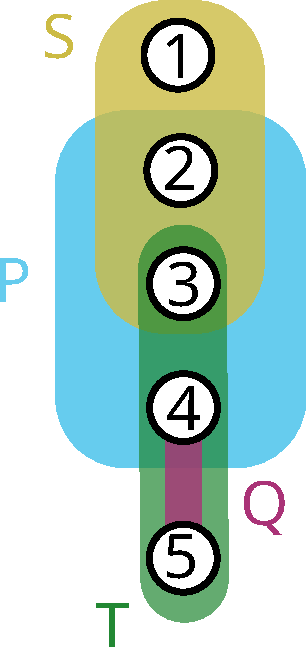
\includegraphics[width=0.9\textwidth]{svg/fgf-unravel.svg/example-struct-1}
    \captionof{figure}{Example structure \struct{A}}\label{fig:fgf-struct-a} \leavevmode\\[-0.5em]
    \raggedright
    $\tups = (1,2,3)$, $\tupp = (2,3,4)$, $\tupt = (3,4,5)$, $\tupq = (4,5)$. \\

    \begin{enumerate}[label=(\arabic*)]
      \item not strict because tail in step from $\tupt$ to $\tupq$ is empty
      \item not strict because step from $\tupp$ to $\tupt$ does not use previous tail
    \end{enumerate}
  \end{minipage}
  }
\end{example}
\end{samepage}

\begin{example}[Traces of paths]
  Traces of some paths from \cref{ex:fgf-paths}:
  {%
    \newcommand{\pA}{{\color{tolbrightYellowDarker}\rho_1}}%
    \newcommand{\pB}{{\color{tolbrightCyanDarker}\rho_2}}%
    \newcommand{\pC}{{\color{tolbrightGreen}\rho_{17}}}%
    \newcommand{\pD}{{\color{tolbrightPurple}\rho_{18}}}%
    \begin{align*}
      \trace{\pA} &= (\pA,1)(\pA,2)(\pA,3) \\
      \trace{\pC} &= (\pA,1)(\pA,2)(\pA,3)(\pC,2)(\pC,3)\\
      \trace{\pD} &= (\pA,1)(\pA,2)(\pA,3)(\pC,2)(\pD,2)\\
      \trace{\pB} &= (\pA,1)(\pA,2)(\pB,2)(\pB,3)
    \end{align*}
  }
\end{example}

\begin{samepage}
\begin{definition}[Trace of a path]
  Let $\rho = \bar{s}_{0}(i_{1}, j_{1})\bar{s}_{1}\cdots{}(i_{n}, j_{n})\bar{s}_{n}$ be a bisimulation path, and $\rho_{\ldots{}k} = \bar{s}_{0}\cdots(i_{k},j_{k})\bar{s}_{k}$ for $0 \le k \le n$ be the k-length prefix of that path.
  The trace of $\rho$ is a sequence of tuples with the following structure, describing the elements traversed by the path:
  \begin{equation*}
  \trace{\rho} = (\rho_{\ldots{}0}, 1)(\rho_{\ldots{}0}, 2)\cdots{}(\rho_{\ldots{}0}, b_{0})(\rho_{\ldots{}1}, a_{1})\cdots{}(\rho_{\ldots{}1}, b_{1})\cdots(\rho_{\ldots{}n}, a_{n})\cdots(\rho_{\ldots{}n}, b_{n})
  \end{equation*}
  where the indices $a_{k}$, $b_{k}$ marking the start and end of each segment are defined as follows:
  \begin{align*}
    a_{0} &= 1                   & b_{n} &= |s_{n}| & \text{edge cases} \\
    a_{k} &= j_{k} - i_{k} + 2    &  b_{k-1} &= j_{k} & \text{for}\ 1 \le k \le n
  \end{align*}

  Every element in a trace has a projection $\pi$ to an element of the original structure.
  This projection is given by:
  \begin{equation*}
    \pi(\rho_{\ldots{}k},x) = s_{k,x}\ \text{for every $0 \le k \le n$}
  \end{equation*}
  The projection $\pi(\trace{\rho})$ of the whole trace is the sequence of the projections of individual trace elements.
\end{definition}
\end{samepage}

\begin{observation}
  If $(\rho,i) \in \trace{\sigma}$ then $\rho \le \sigma$ and $(\rho, i) \in \trace{\rho}$.
\end{observation}

The context of a path represents the elements of the trace which are used in the last step, and is defined as follows:

\begin{definition}[Context of a path]
  For a bisimulation path $\rho = \bar{s}_{0}(i_{1}, j_{1})\bar{s}_{1}\cdots{}(i_{n}, j_{n})\bar{s}_{n}$, the context is defined as: $\context{\rho} = \text{tuple of the last}\ |s_{n}|\ \text{elements of}\ \trace{\rho}$
\end{definition}

Note that $\pi(\context{\rho (i,j) \bar{s}_{n}}) = \bar{s}_{n}$ for any path $\rho$.

\begin{definition}[Bisimilarity of paths]
  Let $\mathfrak{A},\bar{a} \sim_{\textrm{FGF},k} \mathfrak{B}, \bar{b}$ be two bisimilar structures.
  We define $\sim_{\textrm{FGF},k}$ for bisimulation paths inductively as:
  \begin{align*}
    \bar{a} &\sim_{\textrm{FGF},k} \bar{b} & \text{base case} \\
    \rho (i,j) \bar{s} &\sim_{\textrm{FGF,k}} \sigma (i,j) \bar{t} & \text{if}\ \rho \sim_{\textrm{FGF,k}} \sigma \ \text{and}\ \mathfrak{A},\bar{s} \sim_{k-|\rho|} \mathfrak{B},\bar{t}
  \end{align*}
\end{definition}

\begin{observation}\label{obs:path-context-bisim}
  Let $\rho$ and $\sigma$ be bisimulation paths in structures $\mathfrak{A}$ and $\mathfrak{B}$.
  Then $\rho \sim_{\textrm{FGF},k} \sigma$ implies $\mathfrak{A}, \pi(\context{\rho}) \sim_{\textrm{FGF},k+1-|\rho|} \mathfrak{B}, \pi(\context{\sigma})$ and the same holds by induction for any n-length prefixes $\rho_{\ldots{}n}, \sigma_{\ldots{}n}$ of $\rho$ and $\sigma$.
\end{observation}

\begin{definition}[Path-complete tree unraveling]
  For a structure \struct{A}, let $\mathcal{P^{\mathfrak{A}}}_{\bar{a}}$ be the set of all bisimulation paths with start $\bar{a}$.
  The path-complete unraveling $\mathfrak{A}^{*,c}_{\bar{a}}, \bar{a}^{*}$ is the structure with domain $\mathcal{P} \times \mathbb{N}$ (elements of traces).
  Each relation $R_{i}$ is defined in $\mathfrak{A}^{*,c}_{\bar{a}}$ as:
  \begin{equation*}
    R_{i}^{\mathfrak{A}^{*,c}_{a_{0}}} = \left\{ \bar{r} \mid \pi(\bar{r}) \in R_{i}^{\mathfrak{A}}\ \text{and there exists a path $\rho$ with}\ \bar{r} \sqsubseteq \context{\rho}\right\}
  \end{equation*}
  The tuple $\bar{a}$ is lifed to the unraveling as $\bar{a}^{*} = \context{\bar{a}}$.
\end{definition}

\begin{samepage}
\begin{example}\leavevmode\\
    \vspace{0pt}
    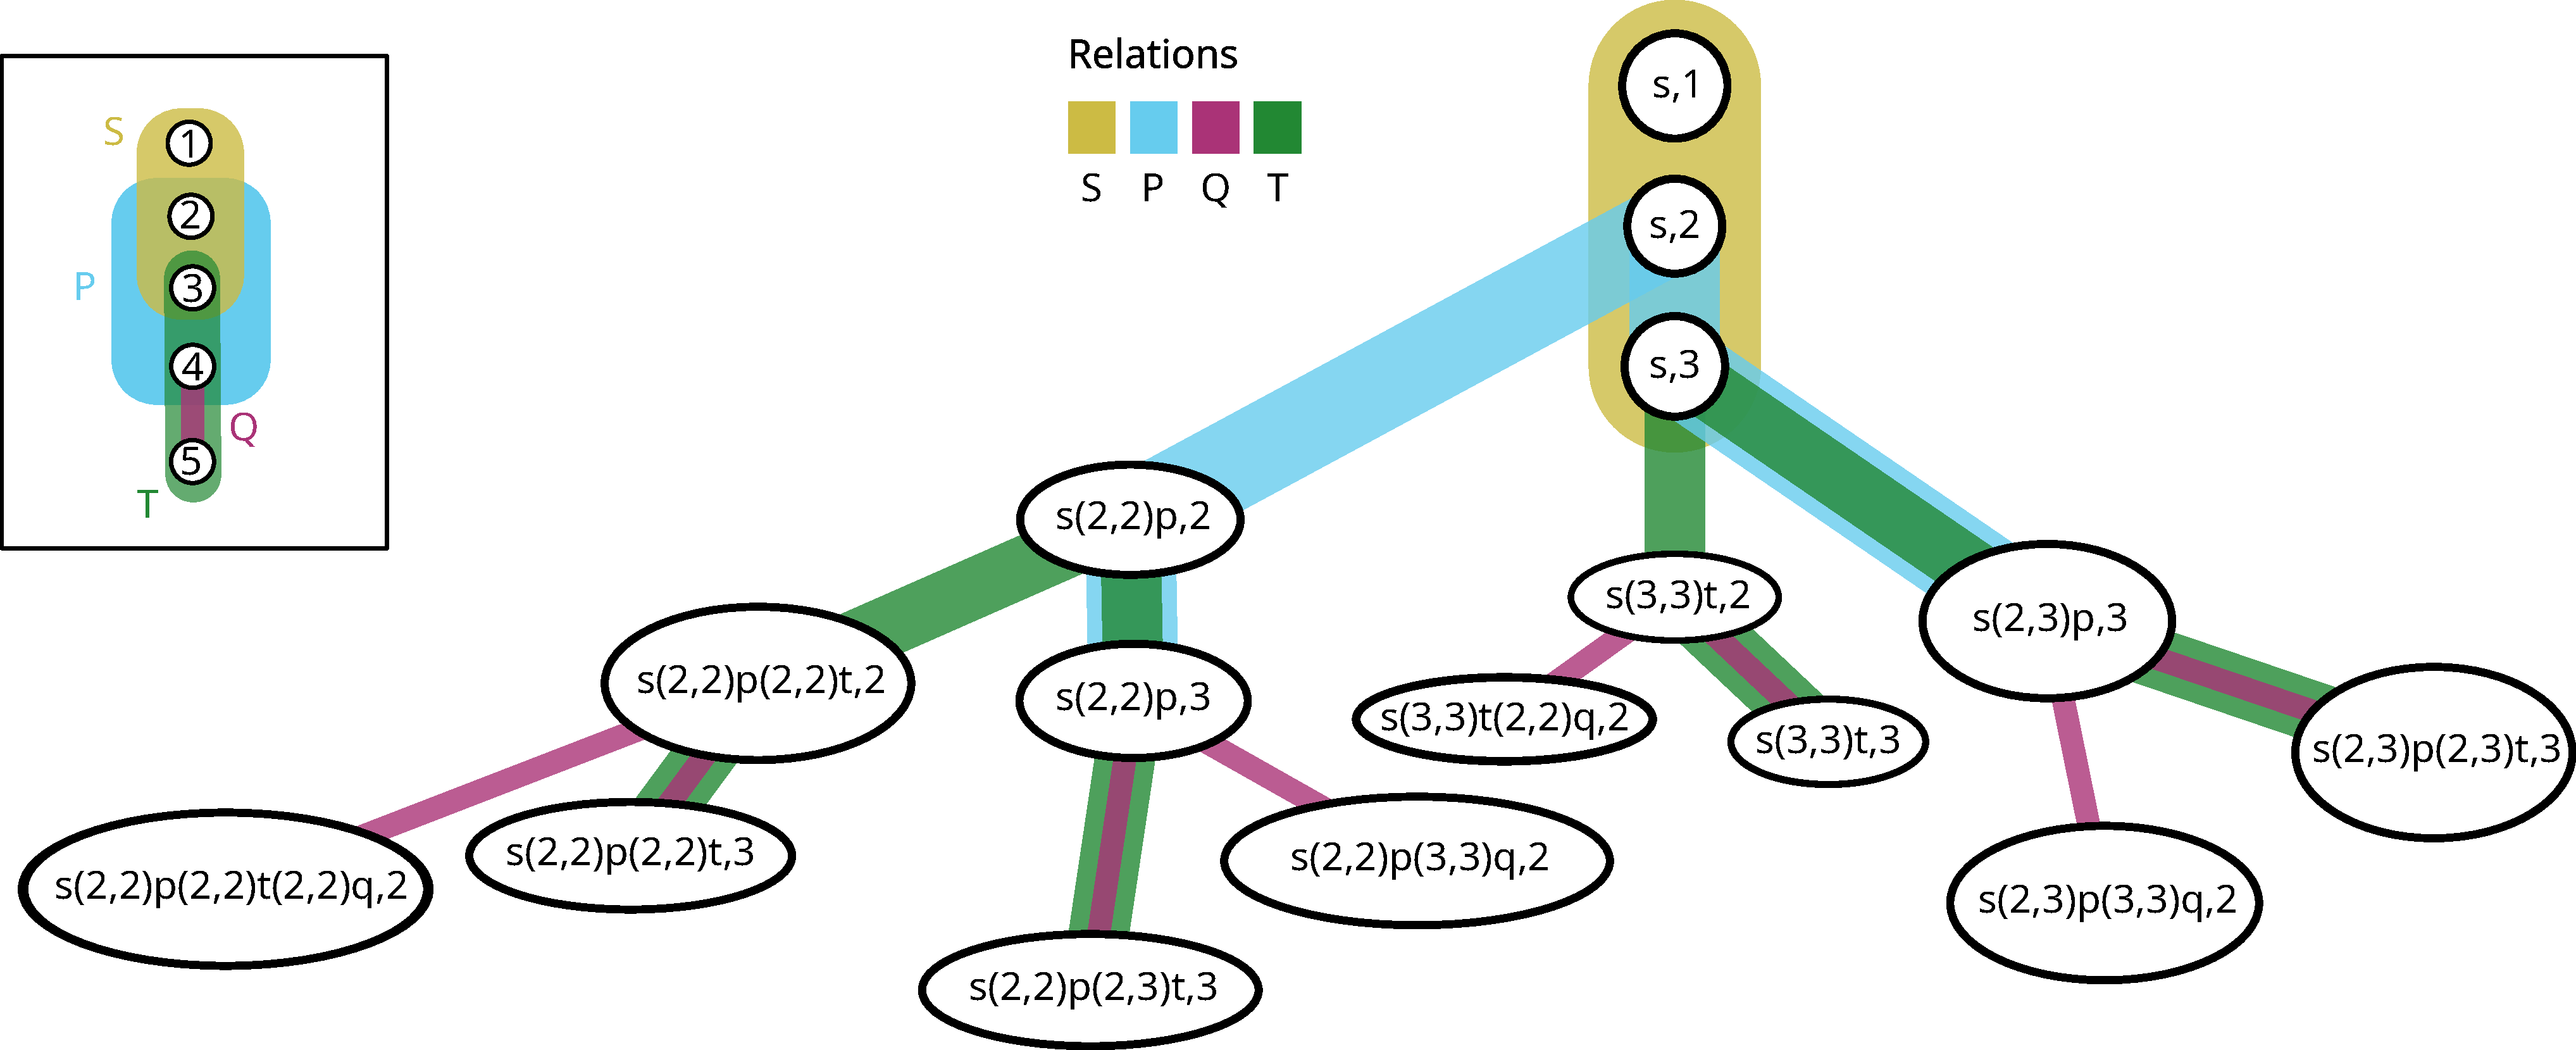
\includegraphics[width=0.9\textwidth]{svg/fgf-unravel.svg/struct-1-unravel}
    \captionof{figure}{Unraveling of structure \struct{A} from \cref{fig:fgf-struct-a}}\label{fig:fgf-struct-a-unravel}
    \vspace{0.5em}
    All starting elements have level 1.
    Every element connected by some relation to those elements has level 2, and so on.
\end{example}
\end{samepage}

\begin{theorem}[$\textrm{FGF}_{k}$ to $\textrm{GF}_{k'}$]
  Let $\mathfrak{A}, \bar{a} \sim_{\textrm{FGF}_{k}}\mathfrak{B}, \bar{b}$ be two connected-forward bisimilar $\Sigma$-structures.
  Then $\mathfrak{A}^{*,c}_{\bar{a}}, \bar{a}^{*} \sim_{\textrm{GF},k'} \mathfrak{B}^{*,c}_{\bar{b}}, \bar{b}^{*}$ for some $k'$ only dependent on $k$ and $\Sigma$.
\end{theorem}

\begin{proof}
  Let $\level{e}$ for $e \in A^{*,c}_{\bar{a}}$ be the length of the shortest path from any element of $\bar{a}^{*}$ to $e$ in the Gaifman graph of the unraveling.
  For a tuple $\bar{s}$, we define $\level{\bar{e}} = \max \level{\bar{e}_{i}}\ \text{for}\ 1 \le i \le |\bar{e}|$.
  We show that a sequence of sets $\mathcal{Z}_{0}, \mathcal{Z}_{1}, \ldots, \mathcal{Z}_{k'}$ form a k'-level connected bisimulation, where each $\mathcal{Z}_{h}$ is defined as follows:
  \begin{equation*}
    \mathcal{Z}_{h} = \left\{
      (\bar{s}, \bar{t})
      \ \middle|\
      \begin{aligned}
        & \text{there are bisimulation paths $\rho$, $\sigma$ such that:} \\
        & \ \text{(a)}\ \rho \sim_{\textrm{FGF}, c*k'} \sigma \\
        & \ \text{(b)}\ \bar{s} = \context{\rho}_{i\ldots{}j}\ \text{and}\ \bar{t} = \context{\sigma}_{i\ldots{}j}\ \text{for some}\ i, j \\
        & \ \text{(c)}\ \level{\bar{s}},\,\level{\bar{t}} \le k' - h + 1
      \end{aligned}
    \right\}
  \end{equation*}

  First we show for any $(\bar{s}, \bar{t}) \in \mathcal{Z}_{h}$ that $\bar{s}, \bar{t}$ induce isomorphic substructures, so the mapping $\bar{s}_{i} \mapsto \bar{t}_{i}$ for $1 \le i \le |\bar{s}|$ is a partial isomorphism.
  Let $\rho$ and $\sigma$ be the paths for $\bar{s}$ and $\bar{t}$ as in the definition of $\mathcal{Z}_{h}$.
  Condition (a) implies by \cref{obs:path-context-bisim} that $\mathfrak{A}, \pi(\context{\rho}) \sim_{FGF,c*k'-|\rho|} \mathfrak{B}, \pi(\context{\sigma})$.
  By the atomic harmony property of FGF bisimulations this means that $\pi(\context{\rho})$ and $\pi(\context{\sigma})$ must have equal forward types.
  This also holds for $\context{\rho}$ and $\context{\sigma}$ since by definition of the unraveling those have the same forward type as the projection.
  Because elements of the unraveling are ordered, substructures with equal forward types are isomorphic.
  As $\bar{s}$ and $\bar{t}$ are simply slices of $\context{\rho}$ and $\context{\sigma}$ they must be isomorphic substructes as well.

  Next we give the proof for \texttt{(gforth)} and \texttt{(gback)} follows by symmetry.
  Let $(\bar{s}, \bar{t}) \in \mathcal{Z}_{h}$ and $\bar{s'} \in \mathfrak{A}^{*,c}_{\bar{a}}$ be a guarded tuple sharing at least one element with $\bar{s}$.
  Since all these tuples are guarded
  \phantom{\qedhere}
\end{proof}

\end{document}
